\section{Результаты}
Были проведены TDDFT-расчеты методом B3LYP/STO-3G. Число МО 56, из них заполнено 34. Число заполненных $\pi$-орбиталей 5 (25, 29-31, 33). Число вакантных $\pi$-орбиталей 5 (35-39). Имеется две $n$-орбитали (32, 34), локализованные на атомах N1 и N2.

\begin{table}[H]
    \caption{Характеристики низних возбужденных состояний}
    \label{tab:my-table}
    \begin{center}
    \resizebox{\textwidth}{!}{%
    \begin{tabular}{|c|c|c|c|c|c|}
    \hline
    \multirow{2}{*}{\begin{tabular}[c]{@{}c@{}}№ низшего\\ возбуждённого состояния\end{tabular}} & \multirow{2}{*}{\begin{tabular}[c]{@{}c@{}}Тип возбужденного\\ состояния\end{tabular}} & \multicolumn{2}{c|}{\begin{tabular}[c]{@{}c@{}}Энергия возбужденния\\ из основного состояния\end{tabular}} & \multirow{2}{*}{\begin{tabular}[c]{@{}c@{}}Конфигурационный\\ состав состояния\end{tabular}} & \multirow{2}{*}{\begin{tabular}[c]{@{}c@{}}Сила осциллятора\end{tabular}} \\ \cline{3-4}
     &  & эВ & см^{-1} &  &  \\ \hline
    1 & $n-\pi$ & 3.225 & 26009.9 & 34 \rightarrow 35 (0.995293) & 0.0028 \\ \hline
    2 & $n-\pi$ & 4.535 & 36576.5 & 34 \rightarrow 36 (0.994412) & 0.0009 \\ \hline
    3 & $n-\pi$ & 4.920 & 39680.3 & 32 \rightarrow 35 (-0.993938) & 0.0006 \\ \hline
    4 & $\pi-\pi$ & 5.036 & 40618.2 & 33 \rightarrow 35 (0.964987) & 0.0688 \\ \hline
    5 & \begin{tabular}[c]{@{}c@{}}$\pi-\pi$\\ $\pi-\pi$\end{tabular} & 5.304 & 42782.9 & \begin{tabular}[c]{@{}c@{}}31 \rightarrow 35 (-0.72705133)\\ 33 \rightarrow 36 (0.672882)\end{tabular} & 0.0019 \\ \hline
    6 & $n-\pi$ & 6.040 & 48716.6 & 34 \rightarrow 37 (-0.978386) & 0.0009 \\ \hline
    \end{tabular}%
    }
    \end{center}
\end{table}

\begin{figure}[H]
    \centering
    \captionsetup{justification=centering}
    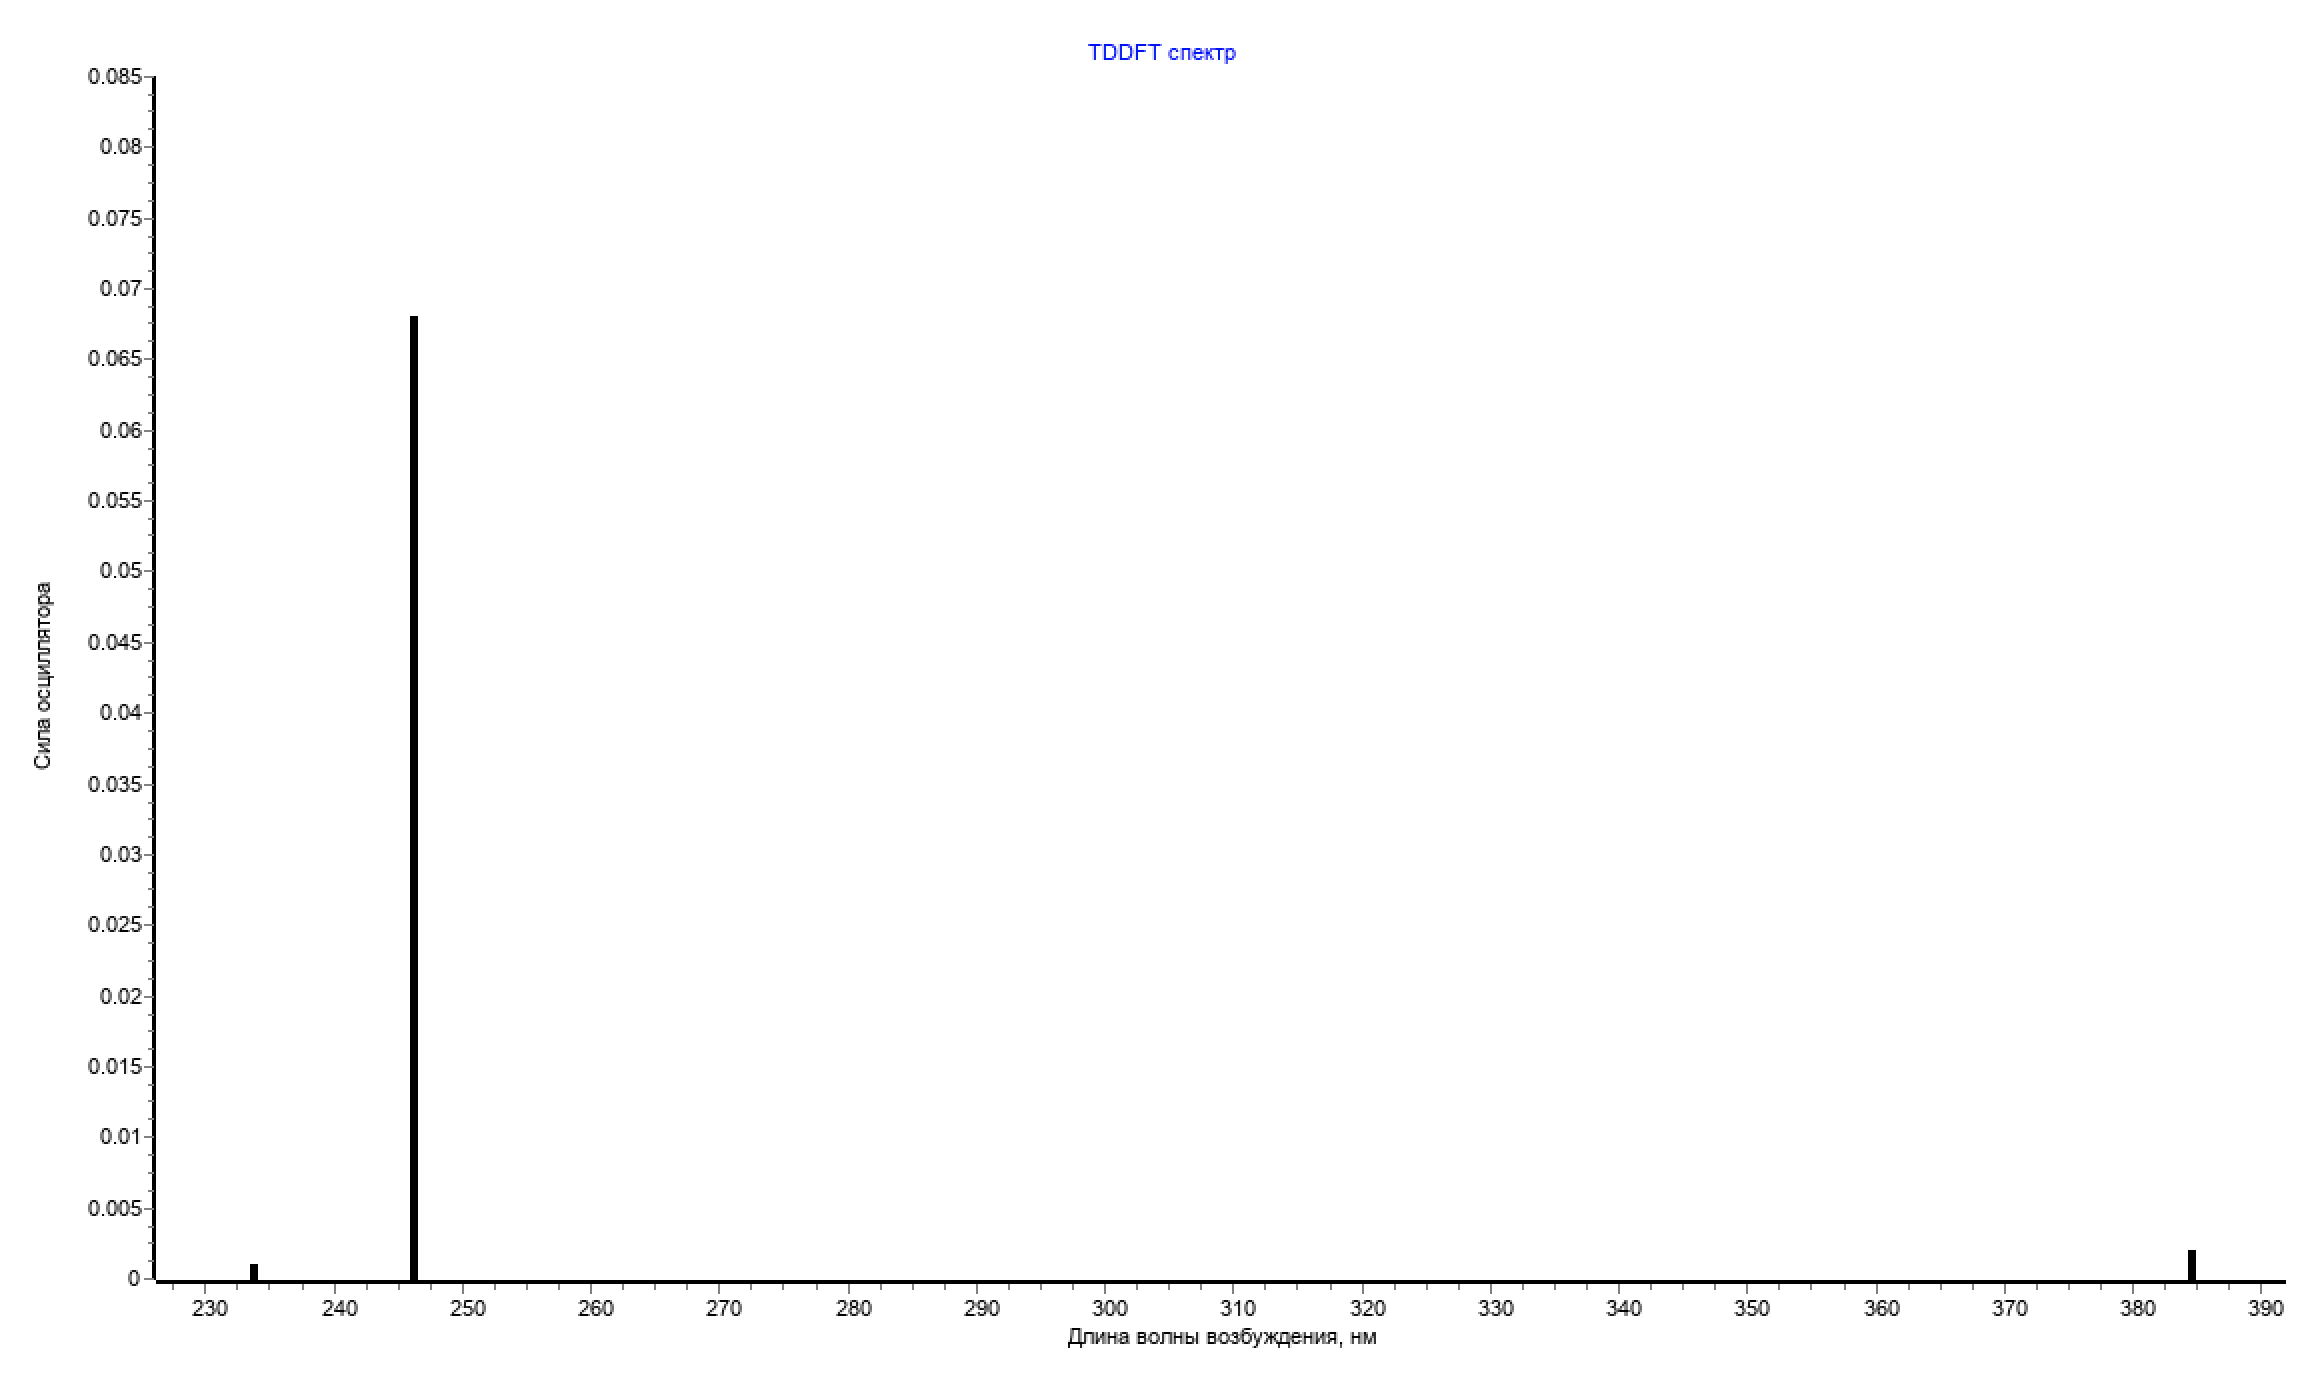
\includegraphics[scale=0.4]{fig/2}
\end{figure}